% Document definition
\documentclass[a4paper,12pt,reqno]{article}

% Elementary packages
\usepackage{graphicx}
\usepackage{amsmath}
\usepackage{amssymb}

\usepackage{caption}

% Things so that the TEX and the HTML look similar
\usepackage{palatino}	% for general text
\usepackage{beramono} 	% for listings

% Colors
\usepackage[usenames,dvipsnames,svgnames]{xcolor}

% Hyper-references
\usepackage[	colorlinks	= true,
			all colors	= NavyBlue!70!Blue	]{hyperref}

% Highlighted box
\usepackage{mdframed}
\mdfsetup{backgroundcolor=yellow!10}
\newenvironment{ybox}{\begin{mdframed}}{\end{mdframed}}

% Listings
\usepackage{listings}

% > Language definition (example)
\lstdefinelanguage{Julia}{morekeywords={abstract,begin,break,case,catch,const,continue,do,else,elseif,end,export,false,for,function,immutable,import,importall,if,in,macro,module,otherwise,quote,return,switch,true,try,type,typealias,using,while},%
   sensitive=true,%
   alsoother={$},%
   morecomment=[l]\#,%
   morecomment=[n]{\#=}{=\#},%
   morestring=[s]{"}{"},%
   morestring=[m]{'}{'},%
}[keywords,comments,strings]%
\lstset{%
    language         = Julia,
    backgroundcolor=\color{Gray!10},
    basicstyle       = \scriptsize\ttfamily,
    keywordstyle     = \bfseries\color{blue},
    stringstyle      = \color{magenta},
    commentstyle     = \color{ForestGreen},
    showstringspaces = false,
}


% newcommands don't have to be here, but cleaner if they are
\newcommand{\bcite}[1]{\href{#1}{\textbf{Link}.}}
\newcommand{\RR}{$\mathbb R$}
\newcommand{\eqa}[1]{\begin{eqnarray}#1\end{eqnarray}}

\title{Example on how to use tex2html}

\begin{document}
\maketitle

\section{Text format}
\subsection{Basics}
\begin{itemize}
    \item Bold: \textbf{bold}
    \item Emph: \emph{emph}
    \item Underline: \underline{underline}
    \item Combo: \textbf{bold \emph{bold emph \underline{everything}} blah}
    \item Color: \textcolor{DarkMagenta}{this in color} (not embeddable)
\end{itemize}

\subsection{References}\\
Hyperreferrences to other sections \hyperref[sec:newcom]{section on newcoms}\\
Referrences to the outside world: \href{http://www.mathjax.org}{\textbf{Link to Mathjax.org}}\\
Referrences to equations: (this shows that you \emph{can} write everything in line, it will be handled but it's not nice, if you write everything out nicely it will also work obviously)
\eqa{ \mathbb I_3 &:=& \left(\begin{array}{ccc}1&0&0\\0&1&0\\0&0&1 \end{array}\right).\label{eq:def id}}
which can then be referred to as \eqref{eq:def id} follows...\\

Raw jem can be inserted at any point (eg., handy for insite short links)
%jem: this a *raw* /jem/ block (see also jemdoc & co)
\section{Environments}
\subsection{Highlighted boxes}
\begin{ybox} This is a highlighted box \end{ybox}

\subsection{Figures}
At the moment, no option allowed (do all that outside, rule of thumb 340x240)
\begin{figure}[!h]\center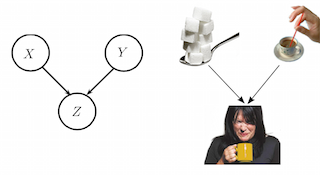
\includegraphics{_figs/vinteractions.png}\end{figure}

\subsection{Equations}
Inline \textbf{small} mode: $4 \ge 3$ is simple inline math\\
Inline \textbf{big} mode:   $$\pi\ge3$$\\
Inline \textbf{big} mode(2) $$\pi\ge3$$\\
Multiline
\begin{eqnarray} 1+1&=&2\end{eqnarray}
Multiline with tag and label
\eqa{
  \sin^2(x)+\cos^2(x) &=& 1, \qquad \forall x\in\mathbb R \tag{A} \label{eq:A}
  % some comment
}
which can then be referred by \eqref{eq:A}, easy enough.\\

Array of equations:
\begin{eqnarray}
    \sin^2(x)+\cos^2(x) - 1 &=& 0\nonumber\\
    |\exp(i\theta)|-1 &=& 0.
\end{eqnarray}

\section{\label{sec:newcom}Using new commands}
Cf definition of some of the newcommands at the beginning of the document:
\begin{itemize}
    \item No arg embedded math: the reals \RR blah
    \item One arg embedded href: \bcite{http://www.openstreetmap.org}
\end{itemize}

\section{Defensive programming}
Empty math: $$ $$ or $ $ or \eqa{}

\end{document}
